\documentclass{article}

\usepackage{graphicx}
\usepackage{polski}
\usepackage{float}

\usepackage[margin=2.5cm]{geometry}


\setlength{\parindent}{0pt}

\title{Raport - czynniki wpływające na zarobki programistów}
\author{Michał Puchyr}

\begin{document}

\begin{titlepage}


    \begin{center}

        \LARGE \textsc{Politechnika Wrocławska}\\
        \vspace*{0.2cm}
        \Large \textsc{Wydział Informatyki i Telekomunikacji}\\
        \vspace*{0.4cm}
        \centering
\includegraphics[width=0.2\textwidth]{WITlogo.png}\\
        \vspace*{0.2cm}
        \vspace*{2cm}

        \centerline{\rule{\textwidth}{1.2pt}}
        \vspace{0.4cm}
        \Huge\textbf{Metody i Systemy Decyzyjne}
        \centerline{\rule{\textwidth}{1.2pt}}
        \vspace{1cm}
        \LARGE Raport - "Co wpływa na wynagrodzenie w branży IT?"\\
        \vspace{3.5cm}
        \textsc{Autor}\\
        \vspace{0.2cm}
        \textbf{Michał Puchyr}\\
        \vspace{0.1cm}
        \Large nr albumu: \textbf{272733}\\
        \vspace{0.1cm}
        kierunek: \textbf{Informatyka Stosowana}

        \vspace*{\fill}
        \Large \textit{\today}

    \end{center}
\end{titlepage}


\section{Problem badawczy}

\textbf{Problem badawczy:} Jakie czynniki wpływają na zarobki programistów w Polsce?

Celem niniejszego raportu jest zbadanie czynników wpływających na zarobki programistów. Rozwój technologii informatycznych sprawia, że programiści są jednymi z najbardziej poszukiwanych pracowników na rynku pracy. W związku z tym, zarobki programistów są bardzo zróżnicowane. W niniejszym raporcie zostaną przedstawione wyniki badań dotyczące zarobków programistów w Polsce oraz czynników, które wpływają na ich wysokość.


\section{Dane badawcze}

Dane potrzebne do przeprowadzenia analizy zostały pobrane z portali NoFluffJobs oraz Pracuj.pl.

\begin{itemize}
    \item Nazwa oferty
    \item Technologie (języki programowania)
    \item Poziom doświadczenia (trainee, junior, mid, senior, expert)
    \item Lokalizacja
    \item Wymagane umiejętności
    \item Zarobki (widełki płacowe - minimalne i maksymalne)
    \item Czy praca jest zdalna
\end{itemize}

\bigskip

Do celów analitycznych zostało pobranych 2859 ofert pracy.
Niestety nie wszystkie oferty zawierały informacje o zarobkach, dlatego zostały one odfiltrowane.

\begin{figure}[h]
    \centering
    \begin{minipage}{0.45\textwidth}
        \centering
        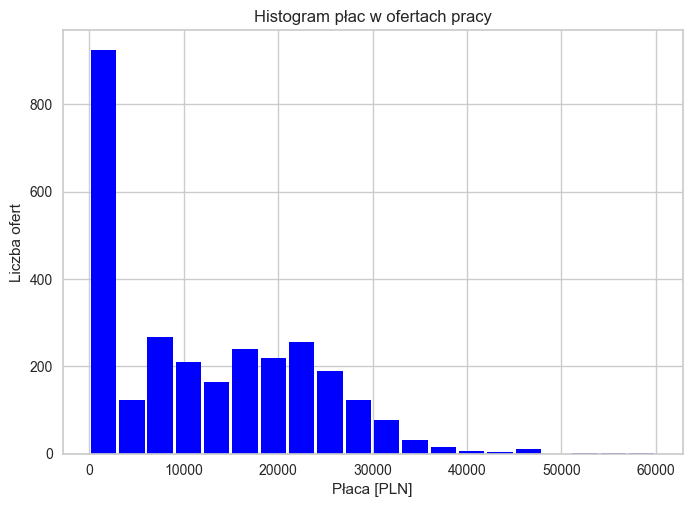
\includegraphics[width=\textwidth]{img/hist_zarobki_z_zerami.png}
        % \caption{Caption for image 1}
    \end{minipage}
    \hfill
    \begin{minipage}{0.45\textwidth}
        \centering
        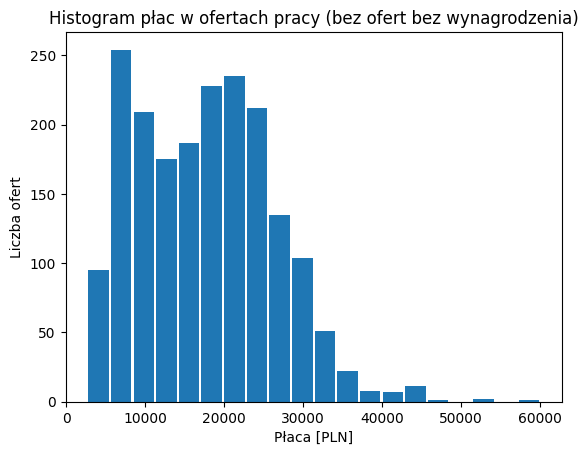
\includegraphics[width=\textwidth]{img/hist_zarobki_bez_zer.png}
        % \caption{Caption for image 2}
    \end{minipage}
\end{figure}

W procesie czyszczenia danych, oferty pracy, które nie zawierały informacji o wynagrodzeniu, miały wartości zerowe w kolumnie zarobków.
Brak danych o zarobkach występuje w około 40\% ofertach pracy, jest to zjawisko zdecydowanie negatywne.
Brak widełek płacowych jest złą praktyką w ogłoszeniach o pracę a z naszego punktu widzenia, uniemożliwia wzięcie oferty pod uwagę w analizie zarobków.
Dobrym pomysłem na osobną analizę jest sprawdzenie, czy brak widełek płacowych jest związany z innymi cechami oferty pracy.
\medskip

Po odfiltrowaniu ofert pracy, które nie zawierały informacji o zarobkach, do dalszej analizy zostało 1937 ofert.

\pagebreak

\section{Analiza danych}

\begin{table}[h!]
    \centering
    \begin{tabular}{|c|c|c|c|c|c|c|c|c|}
        \hline
        & Średnia & Mediana & Odchylenie std. & Min & 25\% & 50\% & 75\% & Maks \\
        \hline
        Zarobki [PLN] & 17637.34 & 17500.00 & 8578.94 & 2664.00 & 10000.00 & 17500.00 & 23520.00 & 60000.00 \\
        \hline
    \end{tabular}
    \caption{Statystyki opisowe zarobków programistów}
    \label{tab:zarobki}
\end{table}

Mediana wysokości płacy analizowanych ofert pracy wynosi 17500 PLN, a średnia 17637.34 PLN.

Odchylenie standardowe wynosi 8578.94 PLN, co oznacza, że zarobki programistów są bardzo zróżnicowane.
Najwięcej ofert pracy możemy znaleźć w przedziale od 10000 PLN do 23520 PLN.
Duża różnica między trzecim a czwartym kwartylem sugeruje, że zarobki powyżej 25 tys. PLN są rzadkością.

\begin{center}
    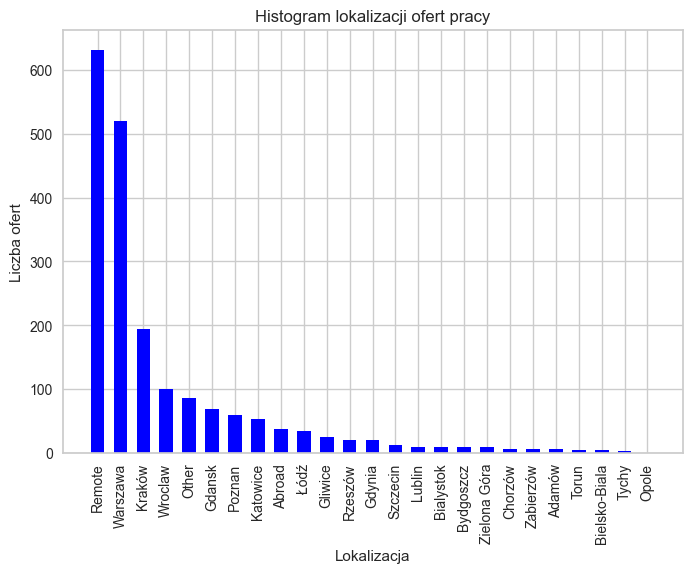
\includegraphics[scale=0.6]{img/location_hist.png}
\end{center}

Najpopularniejszą "lokalizacją" pracy dla programistów jest praca zdalna.
Praca zdalnych jako lokalizacja występuje w 32\% ofert pracy. Jej wpływ na wynagrodzenie
zostanie zbadany w dalszej części raportu.
W przypadku lokalizacji pracy stacjonarnej najwięcej ofert pracy pochodzi z odpowiednio z 
Warszawy, Krakowa, Wrocławia, Gdańska i Poznania co pokrywa się z wielkością tych miast
pod względem liczby mieszkańców.
Do raportu zostały również uwzględnione oferty pracy zza granicy, liczba takich ofert
w porównaniu do ofert z Polski jest znikoma, stanowią one zalediwe 2\% wszystkich ofert,
w związku z czym zostały one wrzucone do jednej kategorii - "Abroad".

\subsection{Wstępne oszacowanie}

Wstępnie możemy dokonać analizy zarobków w zależności od potencjanych czynników.

\begin{figure}[!hbt]
    \centering
    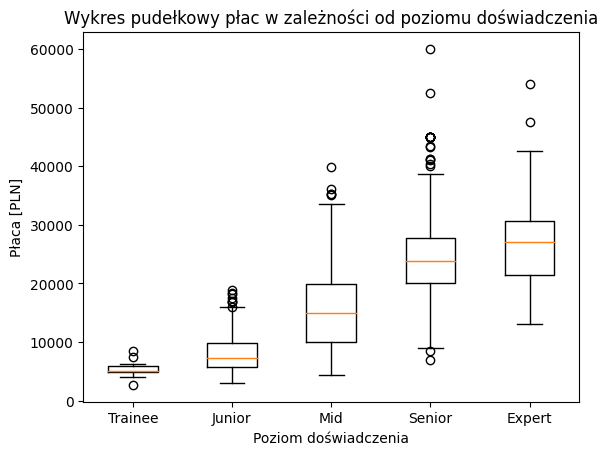
\includegraphics[width=0.7\textwidth]{img/box_zarobki_exp.png}
\end{figure}

\begin{table}[!hbt]
    \centering
    \begin{tabular}{|c|c|}
        \hline
        \textbf{Poziom doświadczenia} & \textbf{Średnie wynagrodzenie [PLN]} \\ \hline
        Expert & 26890.65 \\ \hline
        Senior & 24242.49 \\ \hline
        Mid & 15429.12 \\ \hline
        Junior & 8154.89 \\ \hline
        Trainee & 5232.71 \\ \hline
    \end{tabular}
\end{table}

Z wykresu wynika, że poziom doświadczenia jest wyraźnie skorelowany z wysokością wynagrodzenia co jest zgodne z intuicją.
Im bardziej doświadczony pracownik, tym większą wartość ma jego praca.
Na największe zarobki mogą liczyć programiści klasyfikujący się jako eksperci zaś najmniej jako stażyści i juniorzy.

\begin{table}[H]
    \centering
    \begin{tabular}{|l|r|}
        \hline
        \textbf{Kategoria} & \textbf{Średnie wynagrodzenie [PLN]} \\ \hline
        artificialIntelligence & 27135.55 \\ \hline
        architecture & 25766.50 \\ \hline
        data & 23632.85 \\ \hline
        agile & 22725.00 \\ \hline
        backend & 21734.63 \\ \hline
        \dots & \dots \\ \hline
        hr & 10400.39 \\ \hline
        marketing & 8365.63 \\ \hline
        law & 8186.00 \\ \hline
        officeAdministration & 7807.85 \\ \hline
        customerService & 7166.08 \\ \hline
    \end{tabular}
\end{table}

\textit{Zarobki od 5-tego miejsca od góry do 5-tego miejsca od dołu zostały pominięte w tabeli dla czytelności.}

\medskip

Na najwyższe zarobki przeciętnie mogą liczyć programiści związani z dziedziną sztucznej inteligencji, architekturą oraz danymi.
Najniższe zarobki przeciętnie otrzymują pracownicy związani z obszarami customer service, administracją biurową oraz prawem.

\section{Modelowanie}

Aby móc odpowiedzieć na pytanie o wpływ czynników na zarobki programistów, należy zbadać ważność poszczególnych zmiennych.
W tym celu najlepiej sprawdzi się model regresji liniowej. Poprzez analizę współczynników regresji, można określić, które zmienne mają największy wpływ na zarobki programistów.

\begin{center}
    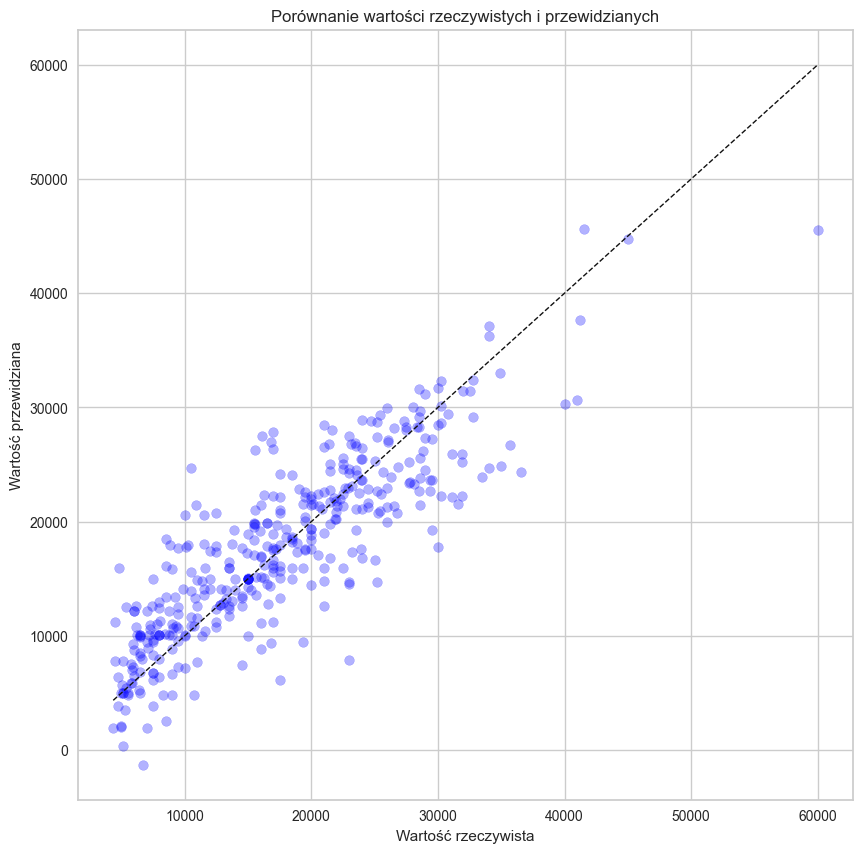
\includegraphics[scale=0.5]{img/model_pred_1.png}
\end{center}

Pod uwagę przy tworzeniu modelu regresji liniowej wzięto następujące zmienne:
\begin{itemize}
    \item Poziom doświadczenia
    \item Technologie
    \item Wymagane umiejętności
    \item Czy praca jest zdalna
\end{itemize}

Score modelu wynosi 73\%, oznacza to, że model, jest w stanie przewidzieć 73\% zmienności wynagrodzenia przez zmienne objaśniające.

Z wykresu również można zauważyć, że dużo jest ofert pracy, których zarobki nie udało się w pełni przewidzieć.
Różnica między wartościami przewidywanymi a rzeczywistymi w pewnych przypadkach jest bardzo duża - rzędu 10 000 złotych.
Jedną z możliwych przyczyn takiego stanu rzeczy jest brak większej liczby danych w zbiorze bądź atrybutów,
które pozwoliłyby wyjaśnić większą część zmienności zarobków programistów.



\end{document}